\documentclass{scrbook}

\usepackage{graphicx}

\usepackage{wrapfig}

\usepackage{multicol}

\title{Patterns}
\author{Firstname1 Lastname1 \and Firstname2 Lastname2 \and Firstname3
Lastname3 \and Firstname4 Lastname4}
\date{\today}


\begin{document}
\frontmatter
\maketitle
\tableofcontents
\mainmatter
\part{Architectural Patterns}
\chapter{Pipes and Filters}
\chapter{Blackboard}
\chapter{Broker}

%Groups I and H
\chapter{Presentation-Abstraction-Control}

\section{Example: Information system for political elections}	%Vera

%TODO Kapitel

The top-level agents abstraction component provides an interface to the data repository, reads, writes and operates on the collected data. The control component organizes communication and cooperation with the intermediate agents. This top-level agent does not have a presentation component. 
There is only one intermediate agent in this example, the view coordinator. Its abstraction component maintains data about all currently active views. Its control component mainly controls and organizes all subordinate agents. It can also create and delete subordinate agents. The presentation component provides a palette of different views from which users can choose one. 
The bottom-level agents control component is responsible for communication with the view coordinator (intermediate agent). Its abstraction component saves the presented data and maintains chart-specific information. The presentation component is responsible for the displaying of the specific chart and providing all functions to be applied on it. 


\section{Context}	%Fabian

%TODO Kapitel

PAC is especially used for developing interactive software. The hierachical structure of PAC suits multi-user
applications well. Systems that experience much replacement, expansion and/or removal of software
components also benefit from the architecture's dynamic design.

\section{Problem}

\begin{multicols}{2}
 



In interactive systems multiple agents work at the same time on separate parts of the same project
(horizontal decomposition). Also, some agents work closer with the database and some of them
closer with the users (vertical decomposition).


\begin{center}
 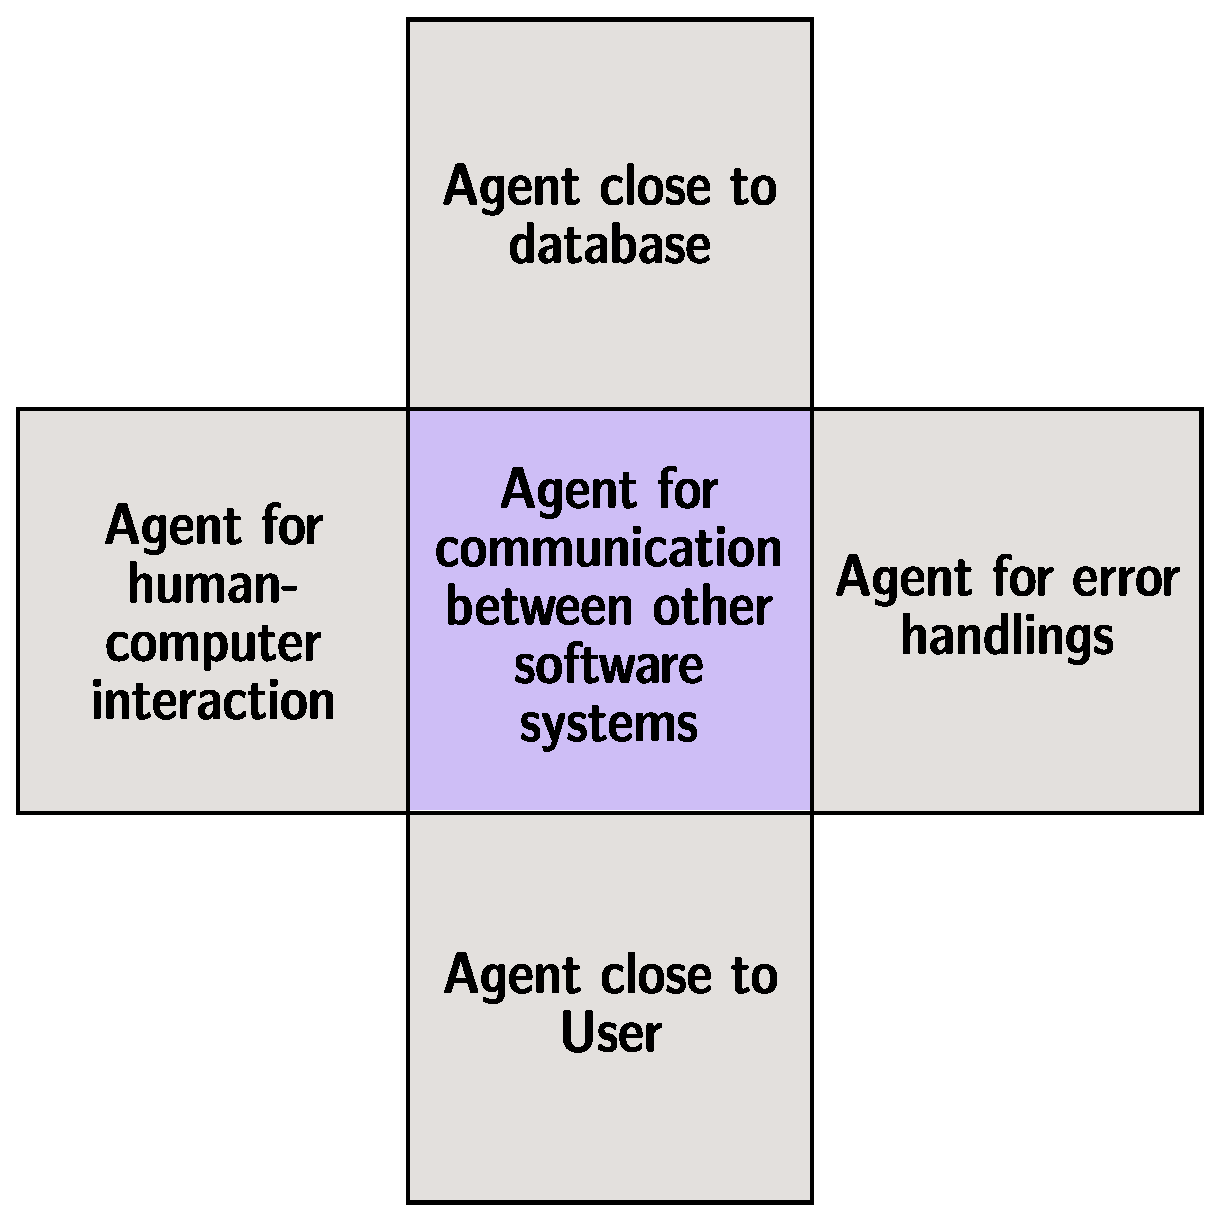
\includegraphics[width=0.4\textwidth]{./pics/problem.eps}\end{center}
 % problem.eps: 0x0 pixel, 300dpi, 0.00x0.00 cm, bb=0 -1 570 570

\end{multicols}

\section{Solution}		%Lucas

The solution consists of handling relations between multiple PAC agents in a tree-like hierarchy. First
of all, every PAC agent is divided into three different components: Presentation, abstraction and
control. The presentation component displays the data to users, while the abstraction component
handles the data model and carries out functional operations on it. The control component primary
connects the presentation and abstraction components and furthermore allows the communication
between its own and other PAC clients.

Now the goal is, to create a structure of multiple PAC agents as the following. There should be one
top-level agent representing the functional core of the whole application, on which most of all the
other agents are depending. As this is the root of our tree, the leaves are called bottom-level agents.
These stand for the interactive part of the system, so users only operate on them. Now intermediate-
level agents are the connection between the functional core and the interactive part of the
application. With these, relationships between and combinations of lower-level agents are
represented.

%TODO Grafik erstellen und einfügen



\section{Structure}	%Jaqueline

To provide the functionality of interactive software systems it is structured as a tree-like hierarchy of
PAC – agents. There are three types of agents (top-level agent, bottom-level agent and intermediate
agent), so “every agent is responsible for a specific aspect of the applications functionality” (cf.
Buschmann et al., Pattern-orientated software architecture: page 146). Agents have three
responsibilities: presentation (graphical user interface), abstract (data model) and control
(communication and mediation between agents).



\subsection{Top-Level Agent}	%Jaqueline

The top-level agent is unique in the system. He accepts all global responsibilities, such as the
database and parts of the user input – interfaces, that cannot be assigned to specific subtasks (cf.
Buschmann et al., Pattern-orientated software architecture: page 147).

The abstraction component of the top-level agent is the interface to all information about the data
model. This includes to manipulate and retrieve information about the data model.
The presentation component of the top-level agent has none, until only a few responsibilities. The
bottom-level agents resume the presentation.

The control component consists of three subcomponents. First, top-level agents allow access to data
model for lower-level agents. Second is the coordination of all PAC agents, to “ensure correct
collaboration and data exchange” (cf. Buschmann et al., Pattern-orientated software architecture:
page 149). Last, a subcomponent is to collect information about interaction between user and
system. The top-level agent checks, if a user request can be performed by data model and
documents history of operations done on the functional core.



\subsection{Bottom-Level Agent}	%Vera

%TODO Kapitel

Bottom-level agents represent one specific object belonging to the application. The presentation component presents a specific view on the object and provides access to functions the user shall be able to use on the object. It also maintains information about the object. The abstraction component is similar to the abstraction component of the top-level agent: it maintains agent-specific data, but no other agent depends on it. The control component manages the relation of presentation component and the abstraction component, serving as an adapter. It is also responsible for communication to intermediate agents, passing outgoing events and messages to the associated higher agents control component and passing incoming events to the presentation component and incoming data to the abstraction component. Bottom-level agents can also provide system services. 


\subsection{Intermediate-Level Agent}

\begin{center}
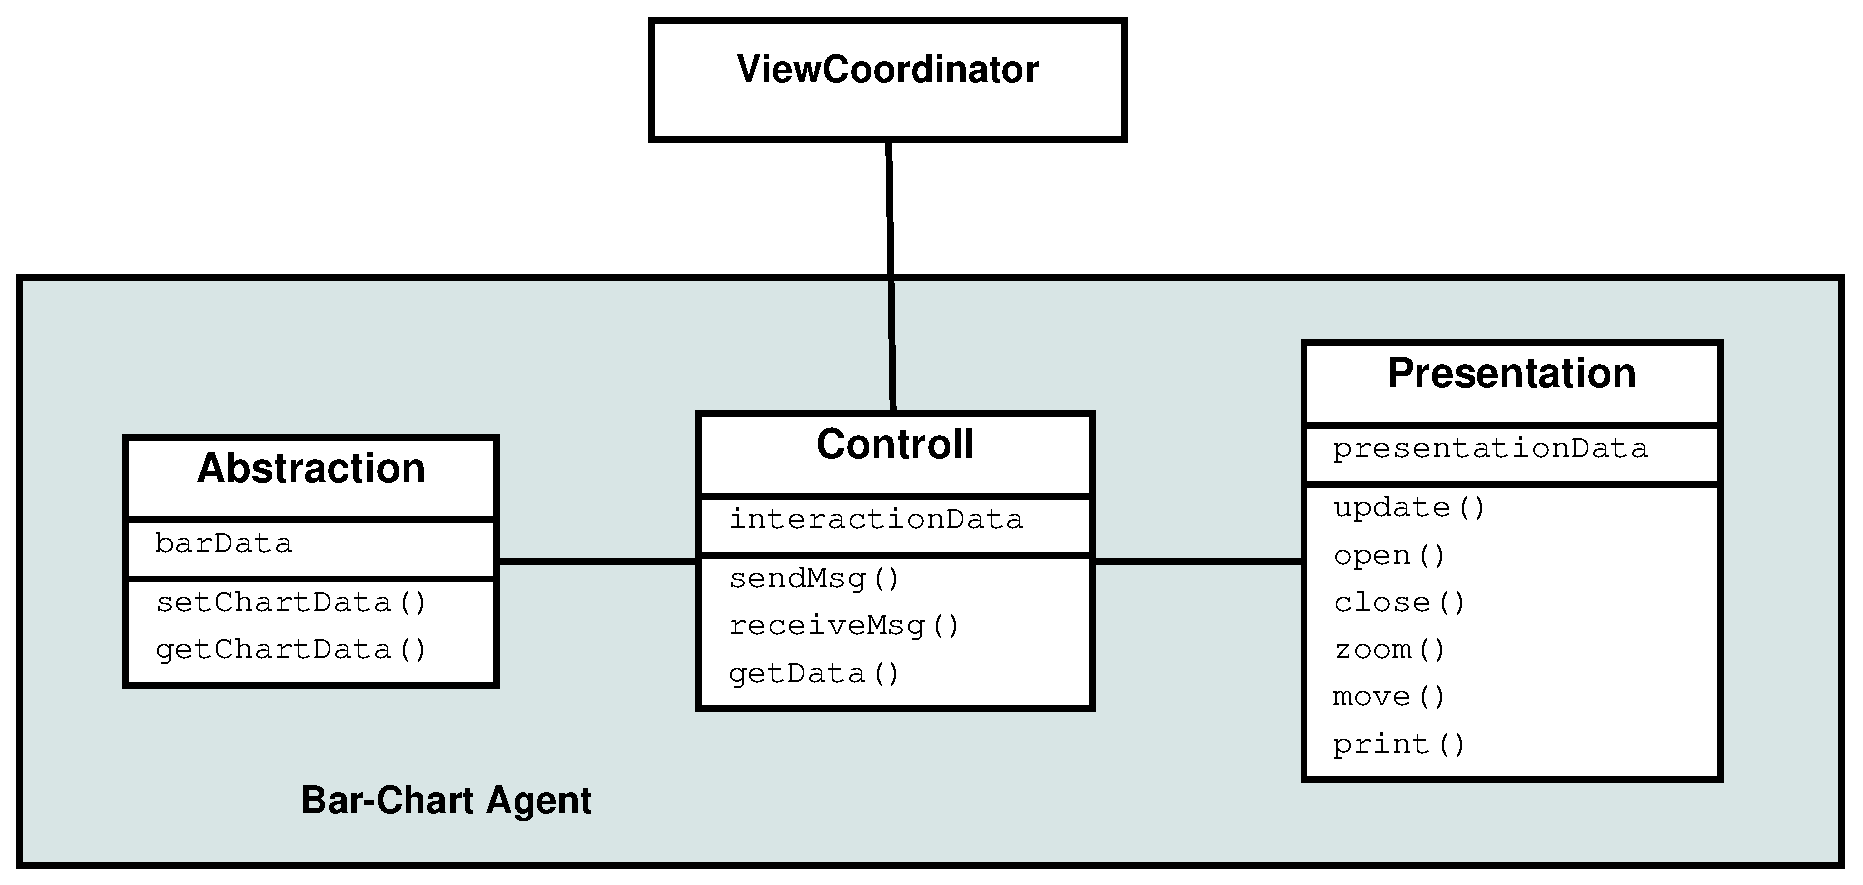
\includegraphics[width=.8\textwidth]{./pics/Components.eps}\end{center}
% Components.eps: 0x0 pixel, 300dpi, 0.00x0.00 cm, bb=0 0 878 409


The intermediate-level PAC agent is responsible for composition and coordination. The agent has to define new abstraction. The other job of the intermediate-level agent is to manage consistency steadiness between the different lower-level agents. 

The abstract component manages the data of the intermediate-level PAC agent. The user interface is implemented by the presentation component. The control component communicates with top-level and bottom-level agents. 

In the information system for political elections we need one intermediate-level agent. The presentation component of the agents creates a tool to view the election data for example in bar or pie charts.  The abstraction component is responsible for all currently active views. Each view is created by one bottom-level agent. The control component must control all subordinate agents. The intermediate-level agent informs the bottom-level agent about changes made by the top-level agent. The intermediate-level agent creates and deflects bottom-level agents on user request. 


\section{Dynamics}	%Nicole

Now we will take a deeper look at the internal functions of PAC, analysing two scenarios.  In the first one we describe what will happen, if a new bar-chart view of the election data is opened.
First a query is send to the presentation component of the view coordinator to open a new bar chart. Then the control of the view coordinator starts the required bar-chart agent. That means the view coordinator sends an open event to the control component of the bar chart agent. At next the control component of the bar chart gets the data from the top-level agent and saves it in the abstraction component. After the process is finished the control component can enable the presentation component to display the chart. At last the presentation component displays a new window with the retrieved data from its belonging abstraction component.

%TODO Bild 1

In the second scenario we have entered new election data in the system.  At first the new data is entered in a spreadsheet and the control component of the spreadsheet agent sends it to the top-level agent. After receiving the spreadsheet the top-level abstraction is requested to change the repository. Then the top-level control component is asked to update all belonging agents with the new data. Therefor we need the view coordinator agent. The view coordinator sends to all view agents a change notification. Now all low-level Agents update their data.  

%TODO Bild 2

\section{Known Uses}

\subsection{Network Traffic Management}
In regular intervals monitored switching units send their traffic data to a control point where the data gets
stored, statistically evaluated and analyzed, and displayed. The data is used to identify problems in the traffic
at which point the system can be used to improve it by changing the networks parameters it displays. The
system is also responsible for handling network exceptions that might occur.

Every single function of the system is represented by its own bottom-level PAC agent. Further PAC agents are
used for each view of the network, the jobs it can perform, and the additional services it offers (e.g. Mail).
Those three categories -view, jobs and additional services- have their own intermediate-level agent that
coordinates their respective bottom-level agents. A forth intermediate-level agent organizes user sessions.
The top-level agent coordinates individual user sessions, and is the only agent to communicate with the
system's functional core. The core is implemented seperately from the agent hierachy.
The hierachy of the system is dynamic. Should, for example, a user start a new session, a corresponding agent
is created. At the end of the session the agent gets deleted.

\subsection{Mobile Root}

The systems purpose is to allow interaction between an operator (user) and a mobile robot. Its mission can be
specified by the operator using this system. The system keeps track of the mission's progress at any time.
The robot navigates itself through a room that can contain walls, equipment and moving obstacles like people.
It does so by using information it receives from both the operator and its built in sensors.

Every wall, route and place is represented by its own bottom-level agent. Together they visualize an
environment which, in turn, is represented by an 'environtment' PAC agent. This agent is at the intermediate
level of the hierachy. These agents control their corresponding bottom-level agents.
The operator can exert control in form of a 'palette' PAC agent that gets implemented, another bottom-level
agent.
Together, a palette and an environment agent form a workplace. Naturally, such a workplace has it's own
agent, also at the intermediate level.
Multiple views of the same environment are handled by a multi-workspace PAC agents.
The top-level agent includes the functional core of the application, which is a rulebased supervisor that
navigates the robot.

\section{Quellen}

%TODO Quellenangaben

%end Groups I and H



\chapter{Microkernel}
\chapter{Reflection}

\end{document}
